% !TEX root = ../main.tex

% 中英标题:\chapter{中文标题}[英文标题]
\chapter{无人机紧急救援系统分析及问题模型构建}[Analysis and Problem Model Construction of UAV Emergency Rescue System]

\section{问题分析}[Problem analysis]
无人机是本课题中所涉及的紧急救援系统的主体,因此在将无人机应用于紧急救援和物资投放时,要综合分析无人机的特点,
在考虑其优势的同时,也要分析其劣势对于救援系统的影响,并在系统设计中做到扬长避短,充分利用无人机本身的特性。


经过综合分析,我们发现无人机在紧急救援系统中,具有以下特点:
\begin{itemize}
	\item [(1)] 
	无人机的续航能力制约了其飞行距离


	\qquad 目前,大多数无人机均采用电池驱动,受制于目前的电池技术发展,民用货运无人机最大历程约为300km,
	且在载重情况下飞行,无人机的续航时间将会进一步降低,同时无人机在电量不足时还需要返回调度中心进行充电\cite{jin2017}。
	\item [(2)]
	无人机相较于大型物资供应车辆,行动更加灵活


	\qquad 自然灾害发生后,受灾地区往往会面临道路中断和交通阻塞等困难。如果使用传统大型物资供应车辆供应物资,
	很有可能会导致紧急物资供应不及时。而无人机在飞行至一定高度后,其行动路径将不会受到上述问题的阻碍,理论上
	可以进行点到点的直接飞行,有效提高了应急救援物资的配送效率\cite{chenhao2019}。
	\item [(3)]
	无人机的飞行受我国法律限制


	\qquad 目前,我国一些地方对于无人机的飞行管理十分严格,设立了禁飞区和管控区等\cite{shu2020},这导致我们在设计无人机紧
	急救援系统时,应该结合实际情况,有效避免无人机的飞行轨迹经过禁飞区。
	\item [(4)]
	民用无人机的载重能力有限


	\qquad 随着无人机技术的不断发展,目前无人机的载重能力已经有了大幅的提升。但是目前重载无人机多用于军事领域,
	在民用领域鲜有使用。因此在设计无人机紧急救援系统时,无人机负责进行的配送物资多为紧急需要的医疗物资和部分
	较轻的生活物资等,在使用无人机进行物资配送时需要考虑这一特点\cite{liuping2016}。
\end{itemize}


在确定使用无人机进行紧急救援任务后,我们还需要对无人机网络通信过程进行分析。
由于目前无人机的应用场景和业务范围较广,国际电信联盟年已经针对民用无人机的通信标准进行立项\cite{hayat2016survey}。
根据无人机的实际任务需求来看,无人机通信中控制命令数据对低延时和高成功率有较高要求,普通环境数据对速率要求较低,一般为kb/s级别,而
实时高清视频的速率要求一般为Gb/s。从飞行距离的角度来看,航拍无人机一般与地面基地的距离约为几十米到上百米,而本问题中涉及到的应急救援无人机与基地的距离可达几十到上百千米级别,相应需要的通信技术
也就从与地面基站直连变为通过移动蜂窝网络(Mobile Cellular Network,MCN)进行通信。移动通信网络的覆盖范围较广,抗干扰性较强,承载的通信容量较高,非常适合无人机进行网络通信\cite{xumin2017}。
目前,中国的4G网络覆盖率已超过98\%,5G网络已覆盖所有地级市城区,超过98\%的县城城区和80\%的乡镇镇区,因此选用4G/5G通信作为无人机网络通信载体是较为合适的方案。

\section{带时间敏感性的无人机网络扫描覆盖问题的建立}[Establishment of Scanning Coverage Problem for UAV Networks with Time Sensitivity]

本课题中提出的无人机紧急救援系统,主要包含了无人机基地、救援点和无人机等,同时还包括无人机调度的优化目标、
约束条件以及求解模型所对应的算法等。该紧急救援系统的总体设计如\figref{fg201}所示:

\begin{figure}[ht]
	\centering
	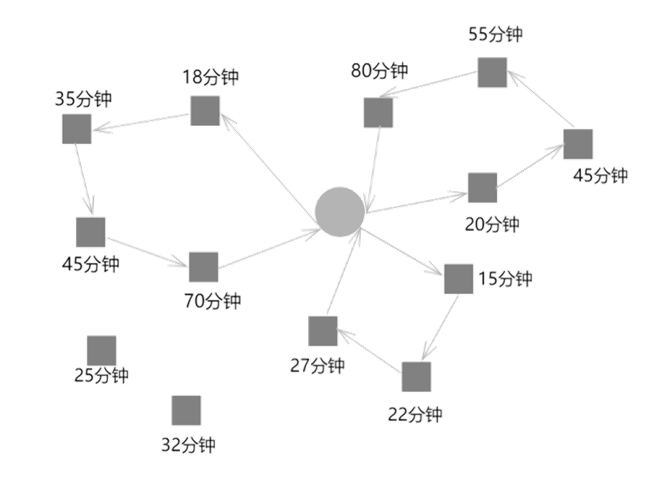
\includegraphics[width = 0.6\textwidth]{fg1_timesensitive}
	\caption{无人机紧急救援系统}
	\label{fg201}
\end{figure}

\begin{itemize}
	\item [(1)]  
	无人机基地和物资仓库(以下简称“基地”)


	\qquad 基地在紧急救援系统中主要负责救援物资的仓储、无人机的调度和无人机的维护充电等工作。当救援物资从
	上游运送到基地后,其能够根据灾区目前的受灾情况和无人机状态等信息,计算和生成无人机调度方案。同时,基地
	也负责对返回基地的无人机进行维护和充电等工作,也是无人机进行起飞和降落的起点和终点。

	\item[(2)]
	救援物资

	
	\qquad 在无人机救援过程中,需要考虑救援物资的质量、大小和配送终点等。在救援物资上印有唯一的身份信息标识,
	基地中的扫描系统可以通过该身份信息标识获取该批救援物资的全部信息,并将这些信息存放在基地的信息管理系统中。

	\item[(3)]
	无人机

	
	\qquad 无人机是课题中紧急救援系统的核心。在无人机执行救援任务时,要对无人机的型号、续航里程、巡航速度和
	最大载重等特性进行研究。民用无人机多用电池续航,采用北斗或GPS导航进行定位,附带有摄像头,可以对救援地点
	进行航拍,以便基地了解受灾地点的现场情况。

	\item[(4)]
	无人机网络通信

	\qquad 在本问题中,无人机通过访问位于公网的服务器与基地间进行数据的相互通信,而无人机访问公网服务器的方式则是通过移动蜂窝网络。
	无人机数据链路根据数据的传输方向可以分为上行链路和下行链路。上行链路主要负责从4G/5G基站到无人机之间控制指令的发送和接收,
	下行链路主要负责无人机到4G/5G基站之间任务完成情况和无人机状态信息的发送和接收。
	

	\item[(5)]
	待救援地点


	\qquad 在救灾过程中,无人机需要在一定时间内快速到达需要被救援的地点,以提供支援。这些地点对于时间要求较为敏感,
	如果无人机不能及时到达,可能会错过最佳救援时机,我们称这些点为兴趣点(Point of Interest,POI)。如\figref{fg201}所示,每个兴趣点都会
	有不同的时间敏感性,如果兴趣点的时间敏感性为15分钟,这意味着这个兴趣点需要在15分钟内被无人机所覆盖。

	\item[(6)]
	问题的优化目标

	\qquad 为了切实保障人民群众生命财产安全,在规划无人机的飞行路径时,应该以实现对更多兴趣点的有效覆盖作为首要目标。
	在实现以上目标的基础上,还需要考虑无人机的调度总成本和飞行距离等因素。在参考了大量有时间窗车辆路径问题
	(Vehicle Routing Problems With Time Windows,VRPTW)后,把主要的优化函数目标概括为:有效覆盖率和准时覆盖率最大化、
	救援成本最小化和无人机的飞行里程最小化,同时满足无人机不超重运输的目标。

	\item[(7)]
	约束条件
	

	\qquad 在VRPTW问题中,需要考虑车辆的载重、运输时间窗和运输完成后车辆必须返回基地等。而当VRPTW问题的主体变为无人机后,
	还需要考虑无人机的续航里程等无人机特有的约束条件。

	\item[(8)]
	问题的求解算法


	\qquad 本文在求解该问题时主要研究了两种算法,一种是改进的贪婪成本选择算法,另一种是改进的遗传算法。在面对简单问题时,贪心式算法
	简单且得到解的速度较快,但当问题较为复杂时,遗传算法是解决该问题的较好选择。
\end{itemize}

\section{无人机紧急救援系统的主要工作流程}[Main workflow of UAV emergency rescue system]
紧急救援系统的主要工作流程如\figref{fg202}所示:

\begin{figure}[ht]
	\centering
	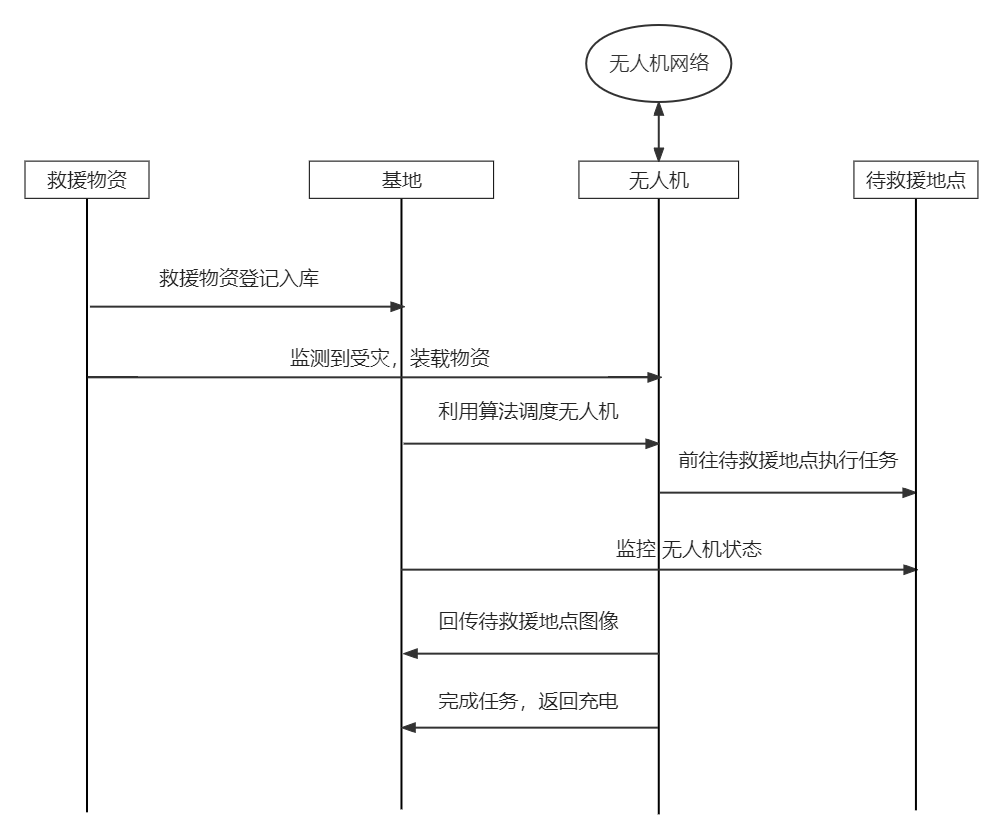
\includegraphics[width = 1.0\textwidth]{fg2_process}
	\caption{无人机紧急救援系统的主要工作流程}
	\label{fg202}
\end{figure}

\begin{itemize}
	\item [(1)]基地在收到新的一批救援物资后,会对救援物资的质量、体积和其他重要信息进行登记造册,存储在基地的物资管理系统中,
	以备查验和后续救援工作使用; 
	\item [(2)]基地的调度中心对无人机的型号、剩余续航时间和载重等信息进行检查,然后根据这些信息,使用算法计算出无人机的最佳调度方案。
	方案中包含无人机的路径规划、运输任务和飞行时间等关键信息;
	\item [(3)]由人工或者智能机器人对无人机进行物资装载,装载完成后,无人机从基地的起降中心出发,开始执行任务;
	\item [(4)]在任务执行过程中,无人机通过网络与基地进行通信,基地可以实时获取无人机的当前状态,同时无人机对拍摄的待救援地点状况进行回传;
	\item [(5)]无人机完成任务后,会与基地调度中心进行确认,待基地确认后,无人机进行返航,本次运送任务结束,待充电完成后准备进行下一次救援任务。
\end{itemize}

\section{问题模型的建立}[Establishment of Problem Model]

\subsection{基地}[Base]
在无人机紧急救援系统的问题模型中,基地使用$B$来表示。当上游救援物资到达基地时,$B$会记录救援物资的详细信息。
基地$B$作为无人机的调度中心和维护中心,会根据获取的信息指挥无人机将物资运送到各个待救援地点。
\subsection{待救援地点及其时间敏感性}[POI]
我们将待救援地点统称为兴趣点,在本问题中,无人机到兴趣点之间的距离与其时间敏感程度无明显关系,因此在设计算法时应该有效协调距离和时间敏感性之间的关系,
并据此对于无人机的路径规划进行决策。假设有$n$个兴趣点,用$P=\lbrace p_1, p_2, \cdots ,p_n \rbrace$进行表示。
这些兴趣点在目标区域内的分布是随机的,位置已知,且为静态。


由于不同的兴趣点其紧急情况不同,它们都有自身的时间敏感性$T_s=\lbrace ts_1, ts_2, \cdots ,ts_n \rbrace$。
我们考虑现实中的实际情况,这些兴趣点可能也会允许无人机在超时一定时间内到达,也将其视为成功救援,
所以我们设置一个公差系数$e$,认为无人机在$(1+e) \cdot t_si$时间内对兴趣点$p_i$进行了救援,即视为救援成功。
\subsection{救援物资}[Relief materials]
在无人机参与应急救援行动前,基地会采集各兴趣点的救援物资需求$S=\lbrace s_1, s_2, \cdots ,s_n \rbrace$, $s_i$代表兴趣点$p_i$所需要的的救援物资的质量。为了简化实验的
研究,我们忽视救援物资的体积,仅考虑救援物资的质量对无人机载重的影响。
\subsection{无人机}[UAV]
基地$B$中停放有$m$架型号相同的无人机,这些无人机用$U=\lbrace u_1, u_2, \cdots ,u_m \rbrace$进行表示,且它们拥有
相同的飞行速度$v$、最大载重$w$、单次飞行载重$w \prime$和最大续航时间$T_{max}$等基础参数。


为了研究的方便,本文在使用无人机执行紧急救援任务时,还对模型进行了适当简化:
\begin{itemize}
	\item [(1)] 无人机以固定速度$v$进行直线飞行,不考虑外界自然条件以及无人机状况对速度的影响;
 	\item [(2)] 不考虑救援物资的体积,只对无人机的载重进行考虑;
  	\item [(3)] 不考虑无人机在起飞和降落过程中对于电量的消耗和花费的时间,无人机从任务开始时即视为已经起飞并离开基地,无人机在完成任务后只要到达基地上方即视为已经返回基地并开始充电。
\end{itemize}

\section{评价指标}[Evaluating indicator]
前面提到,我们在判断无人机是否成功完成对兴趣点的救援时,引入了一个公差系数$e$,认为无人机在$(1+e) \cdot t_si$时间内对兴趣点$p_i$进行了救援,即视为救援成功。所以,我们在评价无人机对兴趣点的覆盖情况时,就有
两项指标:准时覆盖率$R_o$和有效覆盖率$R_e$。
\begin{equation}
R_o=\frac{\sum_{k=1}^m\sum_{i=1}^n o_{ik}}{n}
\end{equation}
\begin{equation}
R_e=\frac{\sum_{k=1}^m\sum_{i=1}^n e_{ik}}{n}
\end{equation}
其中,$o_{ik}$代表第$i$个兴趣点$p_i$是否被第$k$架无人机$u_k$准时覆盖。如果被准时覆盖,则$o_{ik} = 1$,反之$o_{ik} = 0$。
即准时覆盖率是被准时覆盖的兴趣点的数量与所有兴趣点的总数量$n$的比值。


而$e_{ik}$代表第$i$个兴趣点$p_i$是否被第$k$架无人机$u_k$有效覆盖。如果被有效时覆盖,则$e_{ik} = 1$,反之$e_{ik} = 0$。
即有效覆盖率是被有效覆盖的兴趣点的数量与所有兴趣点的总数量$n$的比值。

\section{对问题模型的概述}[Overview of problem model]
经过上面的分析,我们把问题模型定义为:给定一组兴趣点$P=\lbrace p_1, p_2, \cdots ,p_n \rbrace$。这些兴趣点随机地分布在目标区域内,他们拥有自己的时间敏感性$T_s=\lbrace ts_1, ts_2, \cdots ,ts_n \rbrace$
和对救援物资的需求量$S=\lbrace s_1, s_2, \cdots ,s_n \rbrace$。在无人机基地$B$中停放有$m$架无人机$U=\lbrace u_1, u_2, \cdots ,u_m \rbrace$,每架无人机拥有
相同的飞行速度$v$、最大载重$w$、单次飞行载重$w \prime$和最大续航时间$T_{max}$等基础参数。该问题的目标是最大化对兴趣点的准时覆盖率$R_o$和有效覆盖率$R_e$,同时以有效覆盖率$R_e$为最高优先级。
每架无人机在最大续航时间$T_{max}$内完成任务后,都会返回基地$B$,当所有可以被覆盖的兴趣点都完成覆盖后,即视为无人机应急救援任务完成。


对该问题的数学描述如下:

\begin{equation}
 {max}\quad{R_e} 
\end{equation}


从属于:


\begin{equation}
	T_k(i) \le (1+e) \cdot ts_i
\end{equation}
\begin{equation}
	{\forall} k\in \lbrace u_1, u_2, \cdots ,u_m \rbrace ,{\forall} i \in \lbrace p_1, p_2, \cdots ,p_n \rbrace,0\le e \le1
\end{equation}
\begin{equation}
	T_k = \sum_{i=1}^n x_{ik}t_i \le T_{max}
\end{equation}
\begin{equation}
	{\forall} k\in \lbrace u_1, u_2, \cdots ,u_m \rbrace
\end{equation}
\begin{equation}
	w \prime \le w
\end{equation}

\section{本章小结}[Brief summary] 
本章主要建立了无人机紧急救援系统的模型,提出了一套无人机救援任务调度方案,并对整个系统的设计方案和工作流程进行了介绍。
接下来,依次对该系统中的模型进行了介绍,并使用数学符号表示了相关元素,并用数学方式表示了问题中的目标函数和约束等。

